In the previous chapter, we used $\textsc{Max-Cut}$ as a running example to illustrate some derandomisation techniques. In this chapter, we will again look at graph algorithms, but focusing on problems for which we \emph{know} efficient deterministic algorithms. The key message here is that randomisation does allow us to do things \emph{even more efficiently}~--~and, sometimes, to also extract theorems about graphs from our algorithms!

%%%%%%%%%%%%%%%%%%%%%%%%%%%%%%%%%%%%%%%%%%%%%
\section{Karger's Min-Cut algorithm}
We will start with a beautiful algorithm, due to Karger~\cite{Karger93} (and improved by Karger and Stein~\cite{KargerS93}), for the \emph{minimum} cut question:\marginnote{If $G$ is not connected, we can detect this in $O(\orange{m}+\red{n})$ time, and then a ``minimum cut'' is\dots{} easy to find.}
\begin{framed}
\noindent \textsc{Min-Cut}: Given an (undirected) connected graph $G=(\red{V},\orange{E})$ on $\red{n}$ vertices and $\orange{m}$ edges, output a cut $(A,B)$ (partition of $\red{V}$) \emph{minimising} the number $c(A,B)$ of edges between $A$ and $B$.
\end{framed}
Of course, we want an efficient algorithm for that. As a baseline, one could try to ``just'' find a good deterministic algorithm to solve the problem. Fortunately, we have some:
\begin{fact}
    $\textsc{Min-Cut}$ can be solved by computing $\red{n}-1$ instances of the $\textsc{Max-Flow}$ problem.\marginnote{Recall the $\textsc{Max-Flow}$ problem: given a directed weighted graph and two vertices $s$ and $t$, find a maximum feasible flow from $s$ to $t$.} This can be done is polynomial time in $\red{n}$ and $\orange{m}$ (and, actually, in time~\cite{HaoO94} $\bigO{\orange{m}\red{n}\log\frac{\red{n}^2}{\orange{m}}}$).
\end{fact}
This is annoying, as this strongly hints that, well, we're done here. However, the above algorithm is quite involved: can we do as well, or even better, with a \emph{simple} randomised algorithm?

As it turns out, \emph{yes}. Here is the gist of the algorithm: (1)~Pick an edge of the graph uniformly at random. (2)~``Merge'' its two endpoints. (3)~Repeat.

That's all! Of course, to formally describe and analyse this mind-blowingly simple algorithm, we first need to define what we mean by ``merging'' two vertices. This is an operation called \emph{contraction}:
\begin{definition}
    Let $G=(\red{V},\orange{E})$ be a multigraph\footnote{We allow parallel edges, but no self-loops. So there could be several edges between two distinct vertices $u,v$ (but none from $u$ to itself).} and $e=(u,v)\in\orange{E}$ one of its edges. The \emph{contraction of $G$ with respect to $e$}, denoted $G/e$, is the multigraph on $\abs{\red{V}}-1$ vertices defined from $G$ as follows:
    \begin{enumerate}
        \item Replace $u$ and $v$ by a single vertex, $uv$;
        \item Replace all edges of $\orange{E}$ of the form $(u,w)$ or $(v,w)$ by an edge $(uv,w)$;
        \item Remove all self-loops $(uv, uv)$ the second step may have created.
    \end{enumerate}
\end{definition}
The process is illustrated in~\cref{fig:karger:contraction}. Note that a contraction can be performed in time $O(\red{n})$ given either the adjacency list or adjacency matrix representation of the multigraph.
\begin{figure}[htbp]
    \centering
    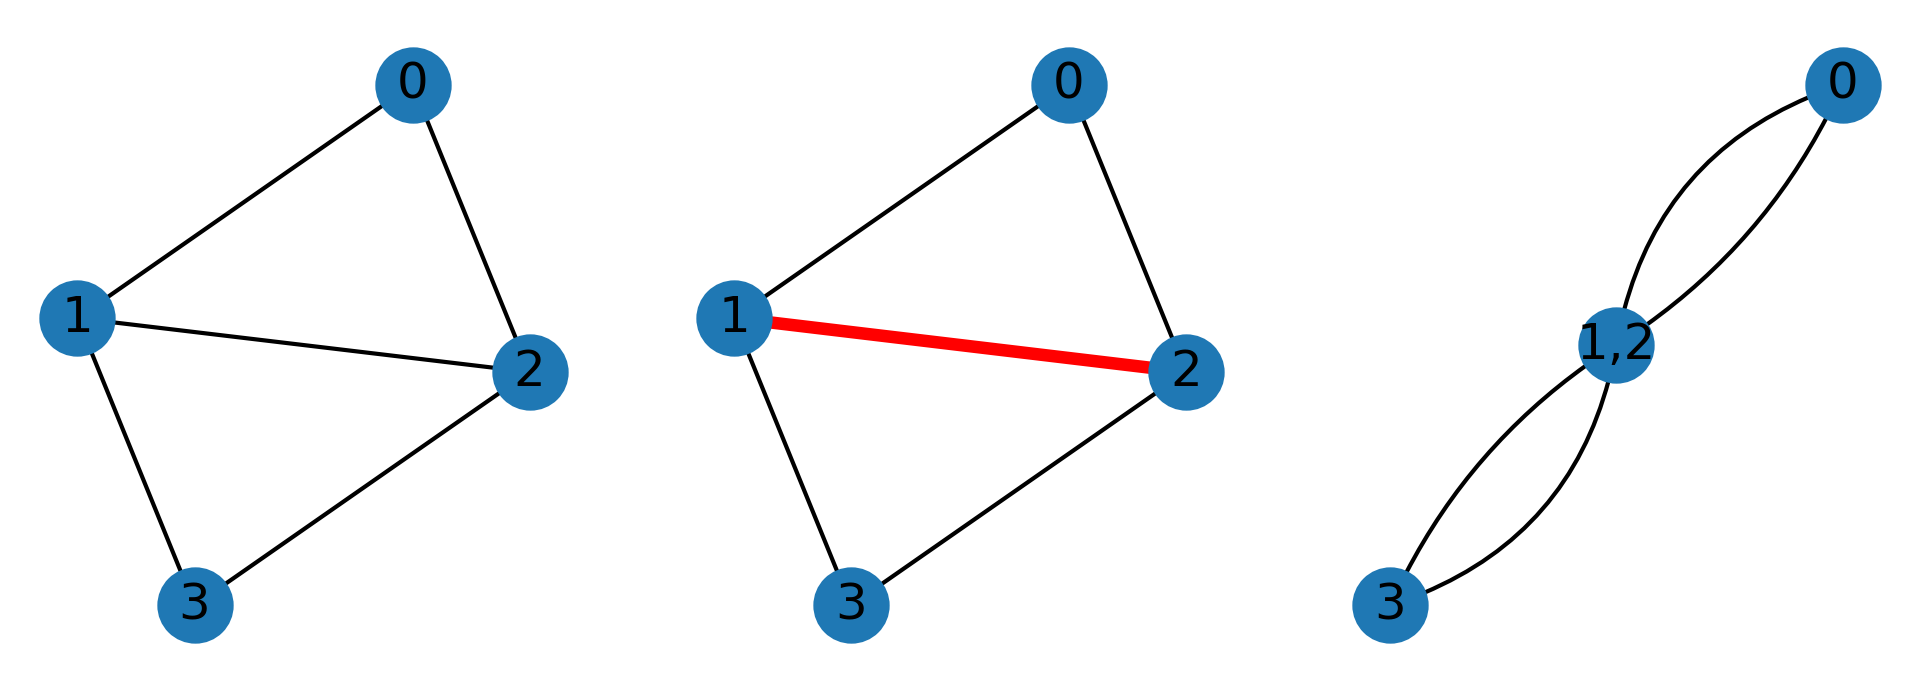
\includegraphics[width=1.0\textwidth]{figures/fig-karger-contraction.png}
    \caption{A contraction of the edge $e=(1,2)$: the original (multi)graph is on the left, and the resulting (multi)graph $G/e$ on the right.}
    \label{fig:karger:contraction}
\end{figure}

Another way to interpret the contraction is that, after contracting some edges to get a multigraph $G'=G/(e_1,\dots, e_k)$, each vertex $u$ in $G'$ corresponds to a subset of vertices $S_u\subseteq \red{V}$ from the original graph $G=(\red{V}, \orange{E})$: the subset of all vertices that were contracted together to become $u$. And any two distinct $u,v$ from $G'$ correspond to \emph{disjoint} subsets $S_v,S_v\subseteq \red{V}$ (during a contraction, a vertex cannot be merged to two separate new vertices!). 

So if after a sequence of contractions we end up with a multigraph $G'$ which has only \emph{two} vertices $u,v$, we get a cut in our original graph $G$: the cut $(S_u, S_v)$. And the value $c(S_u, S_v)$ of this cut is then exactly the number of parallel edges between $u$ and $v$. 

This is the basis for our algorithm, which we are now able to state:
\begin{algorithm}[H]
\begin{algorithmic}[1]
    \Require multigraph $G=(\red{V}, \orange{E})$
    \While{$\abs{\red{V}} > 2$}
        \State\label{alg:krager:randomedge} Pick an edge $e\in\orange{E}$ uniformly at random
        \State\label{alg:krager:result} Contract it, and let $G \gets G/e$
    \EndWhile
    \State\Return the cut defined by the remaining two vertices.
\end{algorithmic}
\caption{Karger's \textsc{Min-Cut} algorithm.}
\label{alg:karger}
\end{algorithm}
This is all. Each iteration of the loop takes time $O(\red{n})$\marginnote{The contraction operation does, and we will see in the tutorial that sampling an edge uniformly can be done in time $O(\red{n})$ as well.}; each contraction reduces the number of vertices by one, and we started with $\red{n}$ vertices: so we have $\red{n}-2$ iterations. Overall, running~\cref{alg:karger} takes $O(\red{n}^2)$ time. \emph{But is the cut it returns any good?} And importantly, \emph{why} would we expect to be any good?

\begin{figure}[htbp]
    \foreach \i in {0,1,...,10}{
    \includegraphics[scale=0.19]{figures/karger/plotgraph-\i.png} 
    }
    \caption{The sequence of steps for one run of Karger's algorithm (\cref{alg:karger}) on a (regular) graph with $\red{n}=12$ vertices and $\orange{m}=48$ edges. The cut returned has $8$ edges.}
\end{figure}

\paragraph{Some intuition.} As a thought experiment, consider any (fixed) cut $C=(A,B)$ of the graph. The only way $C$ will survive until the end of the algorithm (and be returned in~\cref{alg:krager:result}) is if we never contract any edge going from a vertex in $A$ to a vertex in $B$: that is, any vertex of the cut itself. Because as soon as we contract such an edge, some vertex in $A$ is merged with some vertex in $B$, and the cut $(A,B)$ does no longer exist in our new contracted multigraph. Put differently, the more edges there are between $A$ and $B$, the less likely the cut $C$ should be to make it to the end of the algorithm, and as a result, we expect ``small cuts'' (those with fewer edges crossing) to have a better probability to be returned.\marginnote{Consider a different strategy for~\cref{alg:krager:randomedge} of the algorithm, which would sample a pair of distinct vertices $(u,v)$ uniformly at random (not necessarily an edge). Would that work?} But that's exactly what we want: by definition, minimum cuts are the smallest cuts possible! So they should be the ones being the most likely to be returned by our algorithm\dots 

To make it formal, fix any \emph{minimum} cut $C=(A,B)$ of $G$, and let $\green{k}=c(A,B)$ be its value. For $1\leq i\leq \red{n}-2$, let $\mathcal{E}_i$ be the event that the edge $e$ picked in the $i$-th step of the algorithm does \emph{not} belong to our cut $C$. By the above discussion,
\begin{align*}
\probaOf{C\text{ is returned}} 
&= \proba[\mathcal{E}_1\cap \mathcal{E}_2\cap\dots \cap \mathcal{E}_{\red{n}-2}] \tag{No edge from $C$ is ever contracted}\\
&= \proba[\mathcal{E}_1]\probaCond{\mathcal{E}_2}{\mathcal{E}_1}\cdots\probaCond{\mathcal{E}_{\red{n}-2}}{\mathcal{E}_1\cap \mathcal{E}_2\cap\dots \cap \mathcal{E}_{\red{n}-1}}
\end{align*}
Based on this, what we need to conclude is to get a good lower bound on the probability
\[
    \probaCond{\mathcal{E}_{i+1}}{\mathcal{E}_1\cap \mathcal{E}_2\cap\dots \cap \mathcal{E}_{i}}
\]
for all $1\leq i\leq \red{n}-3$: then, we will multiply all of them, and hope for the best. Write $G_i = (\red{V}_i, \orange{E}_i)$ for the multigraph at the end of step $i$: so $G_0=G$, and $G_{\red{n}-2}$ is the $2$-vertex multigraph obtained at the end. The probability that an edge of $C$ is chosen in step $i+1$ to be contracted (if $C$ has survived until then, which is the event $\mathcal{E}_1\cap \mathcal{E}_2\cap\dots \cap \mathcal{E}_{i}$) is then equal to
\begin{equation}
            \frac{\green{k}}{|\orange{E}_{i}|}
\end{equation}
We need to (upper) bound this probability, and all we know is that:\begin{itemize}
    \item the number of vertices is $\abs{\red{V}_i} = \red{n}-i$;
    \item the value of any minimum cut of $G_i$ is $\green{k}$ (there is one cut of size $\green{k}$, our cut $C$ which survived so far; and there cannot be smaller cuts, as they would imply a smaller-than-minimum cut in the original graph $G$ as well).
\end{itemize}
The key observation is that the \emph{minimum degree} of $G_i$ must then be at least $\green{k}$. Otherwise, there would exist some vertex $u\in \red{V}_i$ with less than $\green{k}$ neighbours: choosing the cut $\{u\}, \red{V}_i\setminus\{u\}$ would give a cut in $G_i$ of size less than $\green{k}$. Using the Handshaking Lemma,\footnote{Which, importantly, also holds in (simple) multigraphs.} we have
\begin{equation}
    |\orange{E}_i| = \frac{1}{2}\sum_{v\in \red{V}_i} \deg v \geq \frac{1}{2}\abs{\red{V}_i}\cdot\green{k}
\end{equation}
or, equivalently,
\[
    \frac{\green{k}}{|\orange{E}_i|} \leq \frac{2}{\abs{\red{V}_i}} = \frac{2}{\red{n}-i}\,.
\]
This shows that
\begin{equation}
    \label{eq:karger:proba:failure:step}
    \probaCond{\mathcal{E}_{i+1}}{\mathcal{E}_1\cap \mathcal{E}_2\cap\dots \cap \mathcal{E}_{i}}
    = 1- \frac{\green{k}}{|\orange{E}_i|} \geq 1-\frac{2}{\red{n}-i}
\end{equation}
and as a result, ``multiplying all the conditional probabilities and hoping for the best'' gives
\begin{align}
\probaOf{C\text{ is returned}} 
&= \prod_{i=0}^{\ns-3} \probaCond{\mathcal{E}_{i+1}}{\mathcal{E}_1\cap\dots \cap \mathcal{E}_{i}} \notag\\
&\geq \prod_{i=0}^{\ns-3} \Paren{1-\frac{2}{\red{n}-i}} \notag\\
&= \prod_{i=0}^{\ns-3} \frac{\red{n}-i-2}{\red{n}-i} \notag\\
&= \prod_{j=3}^{\ns} \frac{j-2}{j} \notag\\
&= \frac{1\cdot 2\cdot 3\cdot 4 \cdots (\ns-2)}{3\cdot 4\cdot 5 \cdots \cdot (\ns-2)(\ns-1)\ns} \notag\\
&= \frac{2}{(\ns-1)\ns} \label{eq:karger:success:probability}\,.
\end{align}
What we showed is that, with probability at least $\frac{2}{(\ns-1)\ns}$, Karger's algorithm (\cref{alg:karger}) returns this specific minimum cut $C$. There may be more than one possible minimum cut, so the probability it returns \emph{some} minimum cut is at least $\frac{2}{(\ns-1)\ns}$:
\begin{theorem}
    \label{theo:karger}
    Karger's algorithm (\cref{alg:karger}) returns a minimum cut with probability at least $\frac{2}{(\ns-1)\ns} = \bigOmega{1/\ns^2}$.
\end{theorem}
On the one hand, this is great: the algorithm works! On the other hand, this is somewhat problematic: the probability of success we can guarantee is \emph{very} small. Fortunately, similarly to what we saw in Chapter~2, we can increase our probability of success by repetition, using~\cref{alg:karger} as a blackbox. That is:
\begin{algorithm}[H]
\begin{algorithmic}[1]
    \Require multigraph $G=(\red{V}, \orange{E})$, integer $\blue{T}$
    \For{$1\leq t\leq \blue{T}$} \!\Comment{Use fresh (independent) random bits for each}
        \State Run~\cref{alg:karger} on $G$, let $C_t$ be the output
    \EndFor
    \State\Return the smallest cut among all cuts $C_1,\dots, C_{\blue{T}}$ obtained
\end{algorithmic}
\caption{Amplifying the probability of Karger's \textsc{Min-Cut} algorithm via repetition.}
\label{alg:karger:repeated}
\end{algorithm}
From~\cref{theo:karger}, we know that each of the $\blue{T}$ independent repetitions of the algorithm has probability $p \geq \frac{2}{\ns(\ns-1)}$ of returning a minimum cut. And since it is returning the best cut among them,~\cref{alg:karger:repeated} will return a minimum cut unless \emph{none} of these $\blue{T}$ cuts is a minimum cut. So
\[
    \probaOf{\substack{\text{\cref{alg:karger:repeated} fails to}\\\text{ return a minimum cut}}} = \Paren{1-p}^{\blue{T}} \leq \Paren{1-\frac{2}{\ns(\ns-1)}}^{\blue{T}} \leq e^{-\frac{2\blue{T}}{\ns(\ns-1)}}
\]
where we used the inequality $1-x \leq e^{-x}$ in the end. To achieve probability of success $1-\errprob$, it suffices to choose $\blue{T}$ so that the RHS is at most $\errprob$: one can check that setting 
\[
    \blue{T} = \clg{\ns^2\ln(1/\errprob)}
\]
suffices. Overall, the running time is $O(\blue{T}\ns^2)$, showing the following:
\begin{theorem}
    \label{theo:karger:repeated}
    For any $\errprob>0$, the ``Best-of-$\blue{T}$'' version of Karger's algorithm (\cref{alg:karger:repeated}) returns a minimum cut with probability at least $1-\errprob$, and runs in time $\bigO{\ns^4\log(1/\errprob)}$.
\end{theorem}
Given how simple the algorithm is, this is quite remarkable! However, given that the (much more involved) best deterministic algorithm can find a minimum cut in time $O(\orange{m}\red{n}\log\frac{\ns^2}{\orange{m}}) = \bigO{\ns^3}$, it is natural to wonder if we can do even better. 

\subsection{Improving Karger’s algorithm: the Karger--Stein algorithm} The starting point is to note that Karger's algorithm does \emph{very} well in the first few iterations, but the guarantees degrade quickly towards the end. Again, let's look at a fixed minimum cut $C$ of size $\green{k}$: the probability to ``kill'' $C$ with the first contraction is very small, $\green{k}/\orange{m}$. At the $i$-th step, when $i$ is not too big, this is still very small: in~\cref{eq:karger:proba:failure:step}, we bounded it by
\[
    \frac{2}{\ns-i} \approx \frac{2}{\ns}
\]
All good! But at the \emph{end} of the algorithm, the last few steps, this becomes really, really bad: at the last step ($i=\ns-3$), for instance, the probability that $C$ is ``killed'' is only bounded by
\[
   \frac{2}{\ns-i} = \frac{2}{3} 
\]
This tells us that after surviving almost until the end, we can only guarantee that our minimum cut $C$ has a $33\%$ chance of surviving the very last step! And the first few contractions before that are not much better: each of them has a constant probability of killing $C$.

Based on this, it makes sense to only run Karger's algorithm for a while, and then do ``something else'' once we have contracted sufficiently many edges. This leaves two questions: (1)~When should we stop? and (2)~What should we do afterwards?

To answer the first question, we can look back at our analysis of the success probability. If we stop after $\ns-\blue{s}$ steps, we are left with $\blue{s}$ vertices, and similarly to what we did in~\cref{eq:karger:success:probability} we can guarantee that any fixed minimum cut survives with probability at least
\[
\prod_{i=0}^{\ns-\blue{s}-1} \frac{\red{n}-i-2}{\red{n}-i}
= \prod_{j=\blue{s}+1}^{\ns} \frac{j-2}{j}
= \frac{\blue{s}(\blue{s}-1)}{\red{n}(\red{n}-1)}
\]
If we choose $\blue{s} = \frac{\ns}{\sqrt{2}}+1$, we get
\[
    \probaOf{C \text{ survives these }\ns-\blue{s}\text{ steps}} \geq \frac{1}{2}\,.
\]
So this answers (1): we should stop once only $\frac{\ns}{\sqrt{2}}+1$ vertices remain. Then, even if there was only a single minimum cut $C$ in the original graph, it will have survived with probability at least $1/2$. But turning to question (2): what to do afterwards?\smallskip

We reduced the size of the problem by a constant factor, from $\ns$ vertices to $\approx \frac{\ns}{\sqrt{2}}$. In the absence of a better idea, this seems to call for a recursive approach.\marginnote{``When in doubt, recurse''}

First, the base case: we can only recurse if we make progress at each call, and that can only happen if
\[
    \clg{\frac{\ns}{\sqrt{2}}+1} > \ns
\]
and that is only true for $\ns \geq 7$. This gives us our base case: if $\ns \leq 6$, we will just compute a minimum cut by brute force (in constant time).

Second, $1/2$ probability is much better than $\approx 1/\ns^2$, but it is still small: for a recursive approach, dropping our probability of success by such a constant factor at each recursive step could be bad. But if we have a probability of success at least $1/2$, repeating the first stage \emph{twice} might not be a bad idea: we would have two different multigraphs $G_1,G_2$ on $\blue{s} \approx \frac{\ns}{\sqrt{2}}$ vertices, each of them (independently) still containing a minimum cut with probability at least $1/2$. ``In expectation'', at least $2\cdot (1/2)=1$ still will have a minimum cut. This gives us our algorithm, given in~\cref{alg:karger:stein}.
\begin{algorithm}[htbp!]
\begin{algorithmic}[1]
%%%%%%%%%%%%%%%%%%%%%%%%%%%%%%%%%%%%%%%%%%%%%%%%%%
\algblockdefx{BeginFirstStage}{EndFirstStage}{$\triangleright$~\textbf{Contraction}}{}
\algblockdefx{BeginSecondStage}{EndSecondStage}{$\triangleright$~\textbf{Recursion}}{}
\algtext*{EndFirstStage}% Remove "EndFirstStage" text and line
\algtext*{EndSecondStage}% Remove "EndSecondStage" text and line
%%%%%%%%%%%%%%%%%%%%%%%%%%%%%%%%%%%%%%%%%%%%%%%%%%
\Procedure{ModifiedKarger}{$G=(\red{V}, \orange{E})$, $\blue{s}$}
    \While{$\abs{\red{V}} > \blue{s}$}
        \State Pick an edge $e\in\orange{E}$ uniformly at random
        \State Contract it, and let $G \gets G/e$
    \EndWhile
    \State\Return $G$
\EndProcedure
\Procedure{KargerStein}{$G=(\red{V}, \orange{E})$}
    \If{$\abs{\red{V}} \leq 6$}
        \State \Return a minimum cut \Comment{Brute-force computation}
    \EndIf
    \State Set $\blue{s} \gets \clg{{\ns}/{\sqrt{2}}+1}$
    \BeginFirstStage
        \State $G_1 \gets \textsc{ModifiedKarger}(G,\blue{s})$
        \State $G_2 \gets \textsc{ModifiedKarger}(G,\blue{s})$
    \EndFirstStage
    \BeginSecondStage
        \State $C_1 \gets \textsc{KargerStein}(G_1)$
        \State $C_2 \gets \textsc{KargerStein}(G_2)$
    \EndSecondStage
    \State\label{alg:karger:stein:return}\Return the smallest cut among $C_1,C_2$
\EndProcedure
\end{algorithmic}
\caption{The Improved Karger--Stein \textsc{Min-Cut} algorithm.}
\label{alg:karger:stein}
\end{algorithm}
To analyse this \textsc{KargerStein} algorithm, we need to establish its running time $T(\ns)$ and its probability of success $p(\ns)$. The running time turns out to be the simplest: we have two calls to \textsc{ModifiedKarger}, which (as in~\cref{alg:karger}) each take time $O(\ns^2)$; following by two recursive calls on instances of size $\blue{s}\approx \ns/\sqrt{2}$. Ignoring the ceiling for simplicity, this gives the recurrence relation
\begin{equation}
    T(\ns) = 2T(\ns/\sqrt{2})+O(\ns^2)
\end{equation}\marginnote{Verify it, \eg with the Master Theorem; or, even better, without it.}
which solves to $\boxed{T(\ns)=O(\ns^2\log\ns)}$ \emph{via} the standard techniques.\medskip

The probability of success $p(\ns)$ is trickier. From our setting of $\blue{s}$, we know that $G_1$ still contains a minimum cut with probability at least $1/2$: whenever that happens, $C_1$ will be a minimum cut if the recursive call to \textsc{KargerStein} is successful, which itself happens with probability at least $p(\ns/\sqrt{2})$. That is,
\[
    \probaOf{C_1\text{ is a minimum cut}} \geq \frac{1}{2}\cdot p\Paren{\frac{\ns}{\sqrt{2}}}
\]
Similarly, looking at $G_2$ we have $\probaOf{C_2\text{ is a minimum cut}} \geq \frac{1}{2}\cdot p({\ns}/\sqrt{2})$. Since we are taking the best of $C_1,C_2$ on~\cref{alg:karger:stein:return}, the algorithm succeeds unless \emph{neither} of $C_1,C_2$ is a minimum cut:
\begin{align*}
p(\ns) &= 1-\Paren{1-\probaOf{C_1\text{ is a minimum cut}}}\Paren{1-\probaOf{C_2\text{ is a minimum cut}}} \\
&\geq 1-\Paren{1-\frac{1}{2} p\Paren{\frac{\ns}{\sqrt{2}}}}^2
\end{align*}
We are left with the task of solving this recurrence relation on $p(\ns)$, with the base cases $p(\ns) = 1$ for $\ns\leq 6$. 
\begin{claim}[\advancedstuff]
    The recurrence relation
    \[
       p(\ns) \geq 1-\Paren{1-\frac{1}{2} p\Paren{\frac{\ns}{\sqrt{2}}}}^2
    \]
    has solution $p(\ns) = \bigOmega{1/\log\ns}$.
\end{claim}
\begin{proof}
    Write $\ns = \sqrt{2}^t$ for $t\geq 1$.
    Expanding the square, this boils down to analysing the recurrence relation
    \[
        p(\sqrt{2}^t) \geq p(\sqrt{2}^{t-1}) - \frac{1}{4}p(\sqrt{2}^{t-1})^2
    \]
    or, equivalently (reparameterizing by setting $f(t) = p(\sqrt{2}^t)\in[0,1]$),
    \begin{equation}
        f(t) \geq f(t-1)-\frac{1}{4}f(t-1)^2\,.
    \end{equation}\marginnote{\advancedstuff{} Another ``rabbit-out-of-the-hat'' proof: set $g(t) = \frac{4}{f(t)}-1$, and substitute in the inequality. Solve the resulting inequality.}
    Note that the function $x\mapsto x-\frac{1}{4}x^2$ is increasing on $[0,1]$: this will come handy later. We will show by induction on $t$ that $f(t) \geq \frac{1}{t+2}$.
    \begin{itemize}
        \item This is true for $t=0$, since $f(0) = p(1)=1$.
        \item Assuming it is true for $t-1$, we have
        \begin{align*}
        f(t) &\geq f(t-1)-\frac{1}{4}f(t-1)^2 \\
        &\geq \frac{1}{t+1}-\frac{1}{4}\Paren{\frac{1}{t+1}}^2 \tag{induction hypothesis and $x\mapsto x-\frac{1}{4}x^2$ increasing} \\
        &= \frac{4t+3}{4(t+1)^2} = \frac{1}{t+2} + \frac{3t+2}{4(t+1)^2(t+2)} \\
        &\geq \frac{1}{t+2}
        \end{align*}
        concluding the induction proof.
    \end{itemize}
    Recalling that $\ns = \sqrt{2}^t$, we have $t = 2\log\ns$, and the above shows that $p(\ns) \geq \frac{1}{2\log\ns+2} = \bigOmega{\frac{1}{\log\ns}}$, as claimed.
\end{proof}
\noindent What we have shown can be summarised as follows:
\begin{theorem}
    \label{theo:karger:stein}
    The Karger--Stein algorithm (\cref{alg:karger:stein}) runs in time $O(\ns^2\log\ns)$, and returns a minimum cut with probability at least $\bigOmega{1/\log\ns}$.
\end{theorem}
Moreover, with exactly the same approach as\marginnote{Exercise: prove it!} for~\cref{theo:karger:repeated} (using~\cref{theo:karger:stein} and setting $\blue{T} = O(\log\ns\cdot \log(1/\errprob))$), we get
\begin{corollary}
    \label{theo:karger:stein:repeated}
    For any $\errprob>0$, the ``Best-of-$\blue{T}$'' version of the Karger--Stein algorithm returns a minimum cut with probability at least $1-\errprob$, and runs in time $\bigO{\ns^2\log^2\ns \log(1/\errprob)}$.
\end{corollary}
This is now typically \emph{much} faster than the $\bigO{\orange{m}\red{n}\log\frac{\red{n}^2}{\orange{m}}}$ running time of the deterministic algorithm!\marginnote{Specifically, as long as the graph is even mildly dense, \ie $\orange{m} \gg \ns\log\ns$.}

\begin{remark}
    There is a different deterministic algorithm, due to Stoer and Wagner~\cite{StoerW97} and not based on computing maximum flows, with the running time $\bigO{\orange{m}\red{n}+\red{n}^2\log\red{n}}$ (slightly better than $\bigO{\orange{m}\red{n}\log\frac{\red{n}^2}{\orange{m}}}$, but still worse than~\cref{theo:karger:repeated}). Interestingly, this algorithm also works by performing some type of contraction (merging two carefully selected vertices at each step).
\end{remark}

\subsection{How many minimum cuts are there?}
The \textsc{Min-Cut} question we have considered so far asks to \emph{find} a minimum cut in a graph $G$: \emph{any} minimum cut. There is always at least \emph{one} minimum cut, but could there be more? How many, at most?
\begin{itemize}
    \item $\Theta(\ns)$?
    \item $\Theta(\ns^2)$?
    \item $\Theta(2^{\ns})$?
    \item Something else?
\end{itemize}
And \emph{how to prove it}?\medskip

Fortunately, we already have the answer, \emph{and} done the proof. We just did not realise it at the time! This is a beautiful example where analysing an algorithm establishes a structural result, almost ``as a side effect.''

Taking a step back: in order to prove~\cref{theo:karger}, we have shown that if $C$ is a minimum cut of $G$, then~\cref{alg:karger} outputs $C$ with probability at least
\[
    \frac{2}{\ns(\ns-1)} = \frac{1}{\binom{\ns}{2}}
\]
This means that if there exists $\green{M}$ distinct minimum cuts in the graph $G$, the probability to output one of them is at least
\[
    \probaOf{ \substack{\textsc{Karger}(G)\text{ outputs}\\\text{one of } C_1,\dots, C_{\green{M}}}} = \sum_{i=1}^{\green{M}} \probaOf{ \textsc{Karger}(G)\text{ outputs } C_i} \geq \frac{\green{M}}{\binom{\ns}{2}}
\]
But probabilities are at most one, so $\probaOf{ \substack{\textsc{Karger}(G)\text{ outputs}\\\text{one of } C_1,\dots, C_{\green{M}}}}\leq 1$. Which means that
\[
    \green{M} \leq \binom{\ns}{2}
\]
and we get the following ``for free'':
\begin{theorem}
    An undirected graph $G=(\red{V},\orange{E})$ on $|\red{V}|=\ns$ vertices has at most $\binom{\ns}{2}$ minimum cuts.
\end{theorem}
This is quite surprising, since every\marginnote{Do you see why?}  graph on $\ns$ vertices has exactly $2^{\ns-1}-1$ distinct (not necessarily minimum) cuts. As usual, we can ask whether this $\binom{\ns}{2}$ bound is tight: and the answer is \emph{yes}, as there exist some $\ns$-vertex graphs with that many minimum cuts. A simple example is a cycle on $\ns$ vertices, where choosing any $2$ edges out of $\ns$ defines a distinct minimum cut: see~\cref{fig:cycle:graph}.
\begin{figure}[htbp]
    \centering
    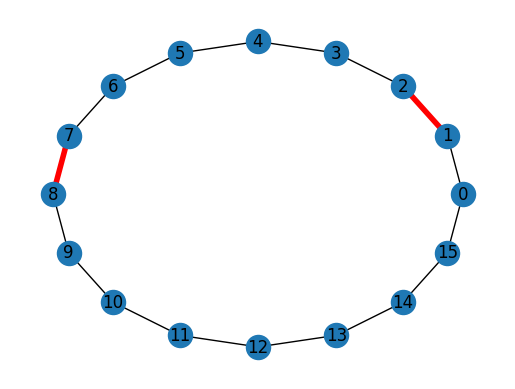
\includegraphics[width=0.9\textwidth]{figures/fig-cyclegraph}
    \caption{The cycle graph $C_{16}$ on $16$ vertices, along with a specific (mininum) cut (defined by the two \red{red} edges). Any choice of two edges creates a different minimum cut of the graph: there are $\binom{16}{2}$ such choices.}
    \label{fig:cycle:graph}
\end{figure}

%%%%%%%%%%%%%%%%%%%%%%%%%%%%%%%%%%%%%%%%%%%%%
\section{Minimum Spanning Tree in Expected Linear Time}
Another classic and fundamental graph problem is the \emph{minimum spanning tree} one, which, given a connected weighted graph $G$, asks to find a spanning tree\marginnote{A \emph{spanning tree} of a graph $G$ is a connected subgraph of $G$ with no cycle. A \emph{spanning forest} is the same thing without the requirement to be connected.} with minimum total weight:\marginnote{A \emph{minimum spanning forest} (MSF) is the equivalent of an MST when the graph is not connected: it asks for a collection of MSTs, one for each connected component of the graph.}
\begin{framed}
\noindent \textsc{Minimum Spanning Tree (MST)}: Given an (undirected) connected graph $G=(\red{V},\orange{E})$ on $\red{n}$ vertices and $\orange{m}$ edges with positive weights $\purple{w}\colon \orange{E}\to \R_+$, output a spanning tree $T$ minimising $\purple{w}(T) = \sum_{e\in T} \purple{w}(e)$.
\end{framed}
As in the previous section, you most likely remember from previous algorithms class that \emph{we have deterministic algorithms to solve this efficiently:}
\begin{itemize}\marginnote{$\log^\ast$ is the iterated logarithm, an incredibly slow-growing function defined as ``the number of times one must apply the logarithm to reach a value at most $1$:''
    \[
        \log^\ast x = \begin{cases}
            0&\text{if } x \leq 1\\
            1+\log^\ast\log x& \text{otherwise.}
        \end{cases}
    \]
    $\log^\ast n$ still goes to infinity as $n$ grows, but \emph{very} slowly.}
    \item Kruskal's algorithm solves it in time $\bigO{\orange{m}\log\red{n}}$
    \item Prim's algorithm solves it in time $\bigO{\orange{m}\log\red{n}}$ when implemented with a heap, or, better, $\bigO{\orange{m} + \red{n}\log\red{n}}$ using a Fibonacci heap
    \item Bor\r{u}vka's algorithm solves it in time $\bigO{\orange{m}\log\red{n}}$
    \item the Fredman--Tarjan algorithm solves it in time $\bigO{\orange{m}\log^\ast\red{n}}$
    \item Chazelle's algorithm solves it in time $\bigO{\orange{m}\alpha(\orange{m},\red{n})}$\marginnote{$\alpha$ is the \emph{inverse Ackermann function}, which grows \emph{even slower}.}
\end{itemize}
The key point is that these algorithms (or their analysis) get more and more involved as we go down the list, and that \emph{no deterministic algorithm running in linear time (that is, $O(\orange{m})$) is known.}\medskip

There is, however, a \emph{randomised} algorithm for MST running in \emph{expected} linear time, due to Karger, Klein, and Tarjan~\cite{KargerKT95}. We will not go through its description and analysis in detail, but will only provide the key building blocks. 

From now on, we will assume for convenience that all the weights $\{\purple{w}(e)\}_{e\in\orange{E}}$ are distinct. This is to make sure we can break ties consistently, and is without loss of generality.\marginnote{A standard way to implement consistent tie-breaking when some weights are equal is to do so using the lexicographic order of the edges.} One nice consequence of this assumption is that the MST is now \emph{unique}: there can be only one!\marginpar{Can you see why?}\medskip

The main idea behind the algorithm can be summarized like this:
\begin{framed}
    \noindent If we had a way to remove most edges from $G$ \emph{without affecting its MST}, then we could recurse on a much sparser graph $G'$.
\end{framed}
The question here is \emph{how} to efficiently remove ``most edges'' (in expectation) without killing the MST in the process.

The first building block we need to answer this are the \emph{cut} and \emph{cycle} properties, which underly the proof (and ideas) behind Prim's and Bor\r{u}vka's algorithm (cut property), and Kruskal's algorithm (cycle property):
\begin{framed}
\noindent\textbf{Cut property.} Let $S\subseteq \red{V}$ be any subset of vertices, and let $e$ be the minimum-weight edge with exactly one endpoint in $S$. Then the MST of $G$ contains $e$.
\end{framed}
\begin{framed}
\noindent\textbf{Cycle property.} Let $C\subseteq \orange{E}$ be any cycle, and let $e$ be the maximum-weight edge belonging to $C$. Then the MST of $G$ does not contain $e$.
\end{framed}
We will require the definition of an edge being ``heavy'' with respect to a forest:
\begin{definition}
    For any weighted graph $G=(\red{V}, \orange{E})$ and forest $F\subseteq\orange{E}$ of $G$, we say that an edge $e\in \orange{E}\setminus F$ is \emph{$F$-heavy} if (1)~adding $e$ to $F$ creates a cycle, and (2)~$e$ is the maximum-weight edge of that cycle.
\end{definition}
\noindent From the cycle property, we readily get the following fact:
\begin{framed}
\noindent\textbf{$F$-heaviness property.} Let $F\subseteq \orange{E}$ be a forest of $G$, and let $e\in \orange{E}\setminus F$ be an \emph{$F$-heavy} edge. Then the MST of $G$ does not contain $e$.
\end{framed}
This looks promising: what this says is that if we have a forest (any forest!) $F$ of $G$, we can safely remove all $F$-heavy edges from $G$ without killing the MST. This sounds exactly like what we are hoping for! Provided, of course, that we can (1)~efficiently find all $F$-heavy edges, and (2)~that there are \emph{many} of them.\smallskip

\noindent The second building block ensures that, at least, we can do (1):
\begin{fact}
    \label{fact:verification:mst}
    There exists a deterministic algorithm $\textsc{MSTVerification}$~\cite{DixonRT92}\cite{King97} which, on input a graph $G=(\red{V}, \orange{E})$ with weights $\purple{w}$ and a forest $F$ of $G$, outputs the set of $F$-heavy edges of $G$ in time $O(\orange{m}+\red{n})$.\marginnote{This type of algorithms is typically used to check whether a given tree is really an MST, hence the name ``MST Verification.''}
\end{fact}

To third and last building blocks will take care of (2). The idea here is that we \emph{already} had the MST $T$ (which we can see as a forest), then by the cycle property \emph{every} edge $e\in G\setminus T$ is $T$-heavy: and so we could use~\cref{fact:verification:mst} on $T$ to find (and remove) $\orange{m}-\red{n}+1$ edges from $G$ in time $O(\orange{m}+\red{n})$. That would be amazing progress~--~but of course, \emph{we do not have $T$}, that's the thing we are trying to compute!

What we \emph{could} do, however, is computing the MST $T'$ of a small random subgraph $G'$ of $G$, and use that as our ``guiding forest'' to find which heavy edges to remove from $G$. If $G'$ has sufficiently few edges and vertices (for instance, $\orange{m}/2$ and $\red{n}/2$) then we can compute its MST $T'$ recursively. So to do that, we need to ``sparsify'' $G$: both in terms of vertices and edges. 

For the edges, this is easy: given a graph $G=(\red{V}, \orange{E})$, we can build a new graph $G'$ with (in expectation) much fewer edges by keeping each edge of $\orange{E}$ independently with probability $\blue{p}\in[0,1]$: this gives us $G'=(\red{V}, \orange{E'})$ with $\expect{|\orange{E'}|} = \blue{p}|\orange{E}|$. Our third building block tells us what happens to the MST\footnote{Or, rather, maximum spanning forest (MSF), since randomly removing some edges might have disconnected $G'$.} when we do that: is the MSF of $G'$ still ``good''?
\begin{lemma}[Random Subsampling Lemma]
    \label{lemma:graph:random:sampling:mst}
    Let $G'=(\red{V}, \orange{E'})$ be a subgraph of $G=(\red{V}, \orange{E})$ obtained by subsampling each edge $e\in\orange{E}$ independently with probability $\blue{p}\in[0,1]$, and $F\subseteq \orange{E'}$ be the MSF of $G'$. Then the expected number of edges \emph{in $G$} that are not $F$-heavy is at most
    $
        \frac{|\red{V}|}{\blue{p}}
    $.
\end{lemma}
We leave the proof of this lemma as an exercise.\marginnote{\advancedstuff{} Exercise!} The crucial part of the statement is that we compute $F$ as the MSF of the \emph{sparser} graph $G'$ but get a guarantee on the number of $F$-heavy edges with respect to the \emph{original} graph $G$.\smallskip

To sparsify $G$ in terms of vertices, the last building block we need is Bor\r{u}vka's algorithm, or, rather, what happens when we run it only for a couple iterations: \cref{alg:boruvka:step}.
\begin{algorithm}[htbp!]
\begin{algorithmic}[1]
\Procedure{BoruvkaStep}{$G=(\red{V}, \orange{E})$, $\blue{t}$}
    \State $F\gets \emptyset$ \Comment{$F$ stands for ``Forest''}
    \For{$1\leq i\leq\blue{t}$}
        \ForAll{$v\in\red{V}$}
            \State Find the lightest edge $e\in\orange{E}$ incident to $v$:
            \[
            e\gets \arg\!\min\{\purple{w}(v,u): (v,u)\in\orange{E}\}
            \]
            \State Contract it, and let $G \gets G/e$
            \State $F\gets F\cup\{e\}$ \Comment{Add it to $F$}
        \EndFor
        \ForAll{$u,v\in \red{V}$} \Comment{In the new graph}
            \If{$u,v$ are connected by more than one edge}
                \State only keep one with the smallest weight
            \EndIf
        \EndFor
    \EndFor
    \State\Return $(G, F)$ \Comment{New graph and forest of contracted edges}
\EndProcedure
\end{algorithmic}
\caption{$\blue{t}$-step version of Bor\r{u}vka's algorithm}
\label{alg:boruvka:step}
\end{algorithm}
\begin{lemma}
    \label{lemma:boruvska:step}
    The $\blue{t}$-step version of Bor\r{u}vka's algorithm, on input a connected graph $G=(\red{V}, \orange{E})$, returns a new graph $G'=(\red{V'}, \orange{E'})$ such that $|\red{V'}| \leq {|\red{V}|}/{2^{\blue{t}}}$, and runs in time $O(\blue{t}\cdot \orange{m})$.
\end{lemma}
\begin{proof}[Proof sketch]
Each step can be implemented to run in time $O(\orange{m})$; and at each step, each vertex is contracted with at least one other, so the total number of vertices decreases by at least a factor $2$.
\end{proof}

\marginnote{Here $\blue{t}\geq 1, \blue{p}\in[0,1]$ are parameters we will get to choose for things to work out.}At this point, we finally have all we need for the algorithm. To summarise our strategy:
\begin{enumerate}
    \item Sparsify $G$ in terms of vertices, to go from $\ns$ to $\ns' = \ns/2^{\blue{t}}$:\marginnote{One can check that adding $F_1$ to an MSF of $G_1$ gives the MST of $G$, so it remains to find an MSF of $G_1$.} this gives a graph $G_1$ on $\ns'$ vertices (and a leftover forest $F_1$ of contracted edges)
    \item\label{step:random:subsampling:mst} Sparsify $G_1$ in terms of edges, to go from $\orange{m}$ to $\orange{m}' \leq \blue{p}\orange{m}$ (in expectation: this is the only random step): this gives a graph $G_2$ on $\ns'$ vertices and $\orange{m}'$ edges
    \item Recursively find the MSF $F_2$ of $G_2$: this should be less expensive, as $G_2$ is smaller than $G$
    \item Find all the $F_2$-heavy edges in $G_1$, and remove them from $G_1$ to get a graph $G_3$: there should be many by~\cref{lemma:graph:random:sampling:mst}, and can be done efficiently by~\cref{fact:verification:mst}
    \item Recursively find the MSF $F_3$ of $G_3$: this should be less expensive, as $G_3$ is smaller than $G$: and this is also the MSF of $G_1$
    \item return $T=F_1\cup F_3$ as the MST of $G$
\end{enumerate}\marginnote{\emph{If} we are lucky, we remove many edges and get $\orange{m}' \ll \orange{m}$ and also end up with many $F_3$-heavy edges, so the recursive calls will be faster. If we are unlucky, the recursive calls will be on bigger graphs, and so will be slower.}
It is worth pointing out that the only random step in the above strategy is Step~\ref{step:random:subsampling:mst}, and it does not affect \emph{correctness}: it only affects the running time.\smallskip

\noindent We can finally state the algorithm itself:
\begin{algorithm}[htbp!]
\begin{algorithmic}[1]
\Procedure{Subsample}{$G=(\red{V}, \orange{E})$, $\blue{p}$}
    \State $\orange{E'} \gets \emptyset$
    \ForAll{$e\in\orange{E}$} \Comment{Independently for each edge}
        \State Add $e$ to $\orange{E'}$ with probability $\blue{p}$
    \EndFor
    \State\Return $G'=(\red{V}, \orange{E'})$
\EndProcedure
\Procedure{LinearTimeMST}{$G=(\red{V}, \orange{E})$, $\blue{t}$, $\blue{p}$}
    \If{$\abs{\red{V}} \leq 2$}
        \Return $G$ \Comment{Base case}
    \EndIf
    \State $G_1 \gets \textsc{BoruvkaStep}(G,\blue{t})$ \label{step:kkt:boruvska}
    \State $G_2 \gets \textsc{Subsample}(G_1,\blue{p})$ \label{step:kkt:subsampling}
    \State $F_2 \gets \textsc{LinearTimeMST}(G_2,\blue{t},\blue{p})$ \Comment{Recursive call}
    \State $H\gets \textsc{MSTVerification}(F_2, G_1)$ \Comment{Find $F_2$-heavy edges} \label{step:kkt:verification}
    \State $G_3 \gets (\red{V_1}, \orange{E_1}\setminus H)$ \Comment{Remove them from $G_1$} \label{step:kkt:pruning}
    \State $F_3 \gets \textsc{LinearTimeMST}(G_3,\blue{t},\blue{p})$ \Comment{Recursive call}
    \State\Return $F_1\cup F_3$
\EndProcedure
\end{algorithmic}
\caption{The Karger--Klein--Tarjan (KKT) Algorithm: MST in expected linear time}
\label{alg:kkt:algorithm}
\end{algorithm}
To analyse it, we need to establish its correctness and expected running time. We will only do the second, as correctness follows from the discussion and lemmas above.\footnote{Please check and establish it, this is a good exercise.}

The expected running time $T(\orange{m},\red{n})$ can be decomposed into the time taken by~\cref{step:kkt:boruvska,step:kkt:verification,step:kkt:pruning}, which by~\cref{fact:verification:mst,lemma:boruvska:step} take total time $O(\orange{m}+\red{n})+O(\blue{t}\orange{m}) = O(\blue{t}(\orange{m}+\red{n}))$; and the time of the two recursive calls, which take time $T(|\orange{E_2}|, |\red{V_2}|) + T(|\orange{E_3}|, |\red{V_3}|)$. Now, $|\red{V_1}|=|\red{V_2}|=|\red{V_3}| \leq \ns/2^{\blue{t}}$ by~\cref{lemma:boruvska:step}, and this is deterministic (comes from the Bor\r{u}vka step); but $|\orange{E_2}|$ and $|\orange{E_3}|$ are random.\marginnote{$|\orange{E_1}|\leq \orange{m}$ but is not necessarily equal to $\orange{m}$, as the Bor\r{u}vka step might have (deterministically) removed a few edges during the contractions.} All we know is that 
\begin{equation}
\label{eq:kkt:bound:expect:E2}
\expect{|\orange{E_2}|}=\blue{p}|\orange{E_1}| \leq \blue{p}\orange{m}
\end{equation}
because of subsampling, and that by~\cref{lemma:graph:random:sampling:mst,lemma:boruvska:step}
\begin{equation}
\label{eq:kkt:bound:expect:E3}
\expect{|\orange{E_3}|} \leq \frac{|\red{V_1}|}{\blue{p}} \leq \frac{\ns}{\blue{p}2^{\blue{t}}}\,.
\end{equation}
So we have, for some absolute constant $C>0$, that
\begin{equation}
    \label{eq:kkt:recurrence}
T(\orange{m},\red{n}) \leq C\cdot \blue{t}(\orange{m}+\red{n})
+ \expect{T(|\orange{E_2}|, |\red{V_2}|)} + \expect{T(|\orange{E_3}|, |\red{V_3}|)}
\end{equation}
where the expectation is over the randomness of the subsampling of the edges (\cref{step:kkt:subsampling}). Let us show by induction that
\[
    T(\orange{m},\red{n}) \leq C'\cdot (\orange{m}+\red{n})
\]
for some suitable constant $C'>0$. The base case is easy, since~\cref{alg:kkt:algorithm} runs in constant time for $\red{n} \leq 2$ (our recursive base case). Now, for the induction, assume this holds for all $(\orange{m},\red{n})$ with $\orange{m'} < \red{m}$ and $\red{n'} < \red{n}$:~\cref{eq:kkt:recurrence} gives
\begin{align}
    T(\orange{m},\red{n})
    &\leq C \blue{t}(\orange{m}+\red{n})
+ \expect{C'(|\orange{E_2}| + |\red{V_2}|)} + \expect{C'(|\orange{E_3}| + |\red{V_3}|)} \notag\\
&\leq C \blue{t}(\orange{m}+\red{n})
+ C'\Paren{\expect{|\orange{E_2}|} + \frac{\red{n}}{2^{\blue{t}}} + \expect{|\orange{E_3}|} + \frac{\red{n}}{2^{\blue{t}}} } \tag{Bound on $|\red{V_2}|,|\red{V_3}|$} \notag\\
&\leq C \blue{t}(\orange{m}+\red{n})
+ C'\Paren{\blue{p}\orange{m} + \frac{\red{n}}{\blue{p}2^{\blue{t}}} + \frac{2\red{n}}{2^{\blue{t}}} } \tag{\cref{eq:kkt:bound:expect:E2,eq:kkt:bound:expect:E3}} \notag\\
&= (C \blue{t}+C'\blue{p})\orange{m} + \Paren{C \blue{t}+C'\frac{2+1/\blue{p}}{2^{\blue{t}}}}\red{n} \label{eq:kkt:recurrence:induction}
\end{align}\marginnote{Check what happens for other choices of $\blue{t}$ and $\blue{p}$: for instance, can you choose $\blue{t}=2$? (This corresponds to only doing two rounds of the Bor\r{u}vka step.) What about $\blue{t}=1$?} %% Comment: for t=2, yes: p = (1+sqrt(5))/4 ~= 0.8 then works. Not t=1.
One can check that setting $\blue{t}=3$, $\blue{p}=1/2$,~\cref{eq:kkt:recurrence:induction} becomes
\begin{align*}
    T(\orange{m},\red{n})
&\leq (3C+C'/2)( \orange{m}+ \red{n} )
\end{align*}
which gives $T(\orange{m},\red{n}) \leq C' ( \orange{m}+ \red{n} )$ as long as $C' \geq 6C$. This concludes the proof by induction, and the proof of the theorem:\footnote{Modulo the parts we left as an exercise.}
\begin{theorem}
    \label{theo:kkt}
    The Karger--Klein--Tarjan algorithm (\cref{alg:kkt:algorithm}) computes a minimum spanning tree (MST) of an $\red{n}$-vertex, $\orange{m}$-edge undirected connected graph in \emph{expected} $\bigO{\orange{m}}$ time.
\end{theorem}
\noindent To conclude, one last thing left as an exercise: can you convert this Las Vegas algorithm into a high-probability Monte-Carlo one?